
%%%%%%%%%%%%%%%%%%%%%%%%%%%%% Define Article %%%%%%%%%%%%%%%%%%%%%%%%%%%%%%%%%%
\documentclass[conference]{IEEEtran}
%%%%%%%%%%%%%%%%%%%%%%%%%%%%%%%%%%%%%%%%%%%%%%%%%%%%%%%%%%%%%%%%%%%%%%%%%%%%%%%

%%%%%%%%%%%%%%%%%%%%%%%%%%%%% Using Packages %%%%%%%%%%%%%%%%%%%%%%%%%%%%%%%%%%
\usepackage{geometry}
\usepackage{graphicx}
\usepackage{amssymb}
\usepackage{amsmath}
\usepackage{amsthm}
    
\usepackage{empheq}
\usepackage{mdframed}
\usepackage{booktabs}
\usepackage{lipsum}
\usepackage{graphicx}
\usepackage{color}
\usepackage{psfrag}
\usepackage{pgfplots}
\usepackage{bm}
\usepackage[spanish]{babel}
\usepackage[utf8]{inputenc} % Codificación UTF-8
\usepackage{amsmath}        % Soporte para ecuaciones matemáticas
\usepackage{graphicx}       % Manejo de imágenes
\usepackage{hyperref}       % Hipervínculos
\usepackage{caption}        % Formato para figuras
\usepackage{multirow}
\usepackage{subcaption}
\usepackage{biblatex}
\usepackage{csquotes}
\usepackage{bookmark}
%%%%%%%%%%%%%%%%%%%%%%%%%%%%%%%%%%%%%%%%%%%%%%%%%%%%%%%%%%%%%%%%%%%%%%%%%%%%%%%

% Other Settings

%%%%%%%%%%%%%%%%%%%%%%%%%% Page Setting %%%%%%%%%%%%%%%%%%%%%%%%%%%%%%%%%%%%%%%
\geometry{a4paper, margin=1in}

%%%%%%%%%%%%%%%%%%%%%%%%%% Define some useful colors %%%%%%%%%%%%%%%%%%%%%%%%%%
\definecolor{ocre}{RGB}{243,102,25}
\definecolor{mygray}{RGB}{243,243,244}
\definecolor{deepGreen}{RGB}{26,111,0}
\definecolor{shallowGreen}{RGB}{235,255,255}
\definecolor{deepBlue}{RGB}{61,124,222}
\definecolor{shallowBlue}{RGB}{235,249,255}
%%%%%%%%%%%%%%%%%%%%%%%%%%%%%%%%%%%%%%%%%%%%%%%%%%%%%%%%%%%%%%%%%%%%%%%%%%%%%%%

%%%%%%%%%%%%%%%%%%%%%%%%%% Define an orangebox command %%%%%%%%%%%%%%%%%%%%%%%%
\newcommand\orangebox[1]{\fcolorbox{ocre}{mygray}{\hspace{1em}#1\hspace{1em}}}
%%%%%%%%%%%%%%%%%%%%%%%%%%%%%%%%%%%%%%%%%%%%%%%%%%%%%%%%%%%%%%%%%%%%%%%%%%%%%%%

%%%%%%%%%%%%%%%%%%%%%%%%%%%% English Environments %%%%%%%%%%%%%%%%%%%%%%%%%%%%%
\newtheoremstyle{mytheoremstyle}{3pt}{3pt}{\normalfont}{0cm}{\rmfamily\bfseries}{}{1em}{{\color{black}\thmname{#1}~\thmnumber{#2}}\thmnote{\,--\,#3}}
\newtheoremstyle{myproblemstyle}{3pt}{3pt}{\normalfont}{0cm}{\rmfamily\bfseries}{}{1em}{{\color{black}\thmname{#1}~\thmnumber{#2}}\thmnote{\,--\,#3}}
\theoremstyle{mytheoremstyle}
\newmdtheoremenv[linewidth=1pt,backgroundcolor=shallowGreen,linecolor=deepGreen,leftmargin=0pt,innerleftmargin=20pt,innerrightmargin=20pt,]{theorem}{Theorem}[section]
\theoremstyle{mytheoremstyle}
\newmdtheoremenv[linewidth=1pt,backgroundcolor=shallowBlue,linecolor=deepBlue,leftmargin=0pt,innerleftmargin=20pt,innerrightmargin=20pt,]{definition}{Definition}[section]
\theoremstyle{myproblemstyle}
\newmdtheoremenv[linecolor=black,leftmargin=0pt,innerleftmargin=10pt,innerrightmargin=10pt,]{problem}{Problem}[section]
%%%%%%%%%%%%%%%%%%%%%%%%%%%%%%%%%%%%%%%%%%%%%%%%%%%%%%%%%%%%%%%%%%%%%%%%%%%%%%%

%%%%%%%%%%%%%%%%%%%%%%%%%%%%%%% Plotting Settings %%%%%%%%%%%%%%%%%%%%%%%%%%%%%
\usepgfplotslibrary{colorbrewer}
\pgfplotsset{width=8cm,compat=1.9}
%%%%%%%%%%%%%%%%%%%%%%%%%%%%%%%%%%%%%%%%%%%%%%%%%%%%%%%%%%%%%%%%%%%%%%%%%%%%%%%

%%%%%%%%%%%%%%%%%%%%%%%%%%%%%%% Title & Author %%%%%%%%%%%%%%%%%%%%%%%%%%%%%%%%
\author{\IEEEauthorblockN{Brayan Joanne Ballesteros Meza, Brayhan Steven Delgado Rueda, Daniel Fernando Aranda Contreras,\\ Jonathan Stiven Murcia Suarez}
\IEEEauthorblockA{Escuela E3T, Universidad Industrial de Santander\\
Correo electrónico: \{brayan2222069, brayan2212088, daniel2221648, jonathan2225092\}@correo.uis.edu.co}}

%%%%%%%%%%%%%%%%%%%%%%%%%%%%%%%%%%%%%%%%%%%%%%%%%%%%%%%%%%%%%%%%%%%%%%%%%%%%%%%
    \begin{document}
        % Título
        \title{\uppercase{Impacto de la selección de la frecuencia de muestreo en la estimación de parámetros de un sistema eléctrico.}}
        \maketitle
        % Resumen
        % Palabras clave        
        \begin{IEEEkeywords}
            Frecuencia de muestreo, Mediciones eléctricas, Análisis de señales, Valor RMS, Muestreo de señales, Errores de estimación, Parámetros del sistema eléctrico, Comparación de procesos de muestreo.   
        \end{IEEEkeywords}

        \section*{Resultados de Medición por Frecuencia Para el Panel de Distrubución} 
        
\subsection*{Tabla T2: Resultados para 180 Hz}
Para este caso de frecuencia de muestreo se consiguen valores con un porcentaje de error del 0.0001\% con relación a los datos obtenidos analíticamente, se aprecia que la frecuencia a la que se esta muestreando es 3 veces el valor de la frecuencia fundamental por lo cual no se incumple el teorema de Nyquist-Shannon.
\begin{table}[h!]
    \centering
    \begin{tabular}{@{}ccccc@{}}
        \toprule
        Vrms [Vrms] & Irms [Arms] & P [W] & Q [VAR] & S [VA] \\ \midrule
            110 & 11.0293 & 1155.1 & 371.1589 & 1213.2\\ 
            \bottomrule
    \end{tabular}
    \caption{Resultados medidos a 180 Hz.}
\end{table}



\subsection*{Tabla T2: Resultados para 200 Hz}
Para este caso es posible conseguir valores mas precisos, se requería de tres ventanas de observación de las cuales solo se están usando dos para tomar medidas y además de eso diez medidas de las cuales solo tenemos información de seis en esas dos ventanas de observación.
\begin{table}[h!]
    \centering
    \begin{tabular}{@{}ccccc@{}}
        \toprule
        Vrms [Vrms] & Irms [Arms] & P [W] & Q [VAR] & S [VA] \\ \midrule
        118.8136 & 11.7527 & 1155.1 & 784.6681 & 1396.4 \\ 
        \bottomrule
    \end{tabular}
    \caption{Resultados medidos a 200 Hz.}
\end{table}

\subsection*{Tabla T3: Resultados para 240 Hz}
Para este caso de frecuencia de muestreo se consiguen valores con un porcentaje de error del 0.0001\% exactamente igual a la frecuencia de 180 [Hz]. Con relación a los datos obtenidos analíticamente, se aprecia que la frecuencia a la que se esta muestreando es 4 veces el valor de la frecuencia fundamental por lo cual no se incumple el teorema de Nyquist-Shannon. 

\begin{table}[h!]
    \centering
    \begin{tabular}{@{}ccccc@{}}
        \toprule
        Vrms [Vrms] & Irms [Arms] & P [W] & Q [VAR] & S [VA] \\ \midrule
        110.0000 & 11.0293 & 1155.1 & 371.1590 & 1213.2 \\ 
        \bottomrule
    \end{tabular}
    \caption{Resultados medidos a 240 Hz.}
\end{table}

\subsection*{Tabla T4: Resultados para 280 Hz}
Similar al caso de la frecuencia de 200 Hz para este se requería de catorce muestras de las cuales solo se tienen nueve, además de eso se requería de tres ventanas de observación de las cuales solo se tienen dos.
\begin{table}[h!]
    \centering
    \begin{tabular}{@{}ccccc@{}}
        \toprule
        Vrms [Vrms] & Irms [Arms] & P [W] & Q [VAR] & S [VA] \\ \midrule
        116.6726 & 11.5761 & 1155.1 & 699.9905 & 1350.6  \\ 
        \bottomrule
    \end{tabular}
    \caption{Resultados medidos a 280 Hz.}
\end{table}

\subsection*{Tabla Final: Resultados para 100 Hz}
Finalmente en este caso se da antialiasing, puesto que la frecuencia de muestreo de la señal es menor al doble de la frecuencia fundamental de la red.
\begin{table}[h!]
    \centering
    \begin{tabular}{@{}ccccc@{}}
        \toprule
        Vrms [Vrms] & Irms [Arms] & P [W] & Q [VAR] & S [VA] \\ \midrule
        118.8136 & 13.2088 & 1155.1 & 1062.5 & 1569.4 \\ 
        \bottomrule
    \end{tabular}
    \caption{Resultados medidos a 100 Hz.}
\end{table}
	
        
\section*{Factor de Potencia (FP) y Potencia Activa Consumida por el Parlante}

\begin{table}[h!]
\centering
\begin{tabular}{ccc}
\toprule
\textbf{Frecuencia [Hz]} & \textbf{FP (Factor de Potencia)} & \textbf{($P_{\text{parlante}}$) [W]} \\
\midrule
100  & 0.7361 & 1129.2 \\
180  & 0.9521 & 1129.2 \\
200  & 0.8272 & 1129.2 \\
240  & 0.9521 & 1129.2 \\
280  & 0.8552 & 1129.2 \\
\bottomrule
\end{tabular}
\caption{Resultados de FP y potencia activa consumida por el parlante para diferentes frecuencias.}
\label{table:resultados}
\end{table}

        \section{Modelo del circuito}

Para el circuito de la Figura \ref{fig:mi_imagen} se tiene que la corriente $I$ es la misma en todas las ramas
    

\begin{figure}[h] % 'h' indica que la imagen se coloca aquí
    \centering
    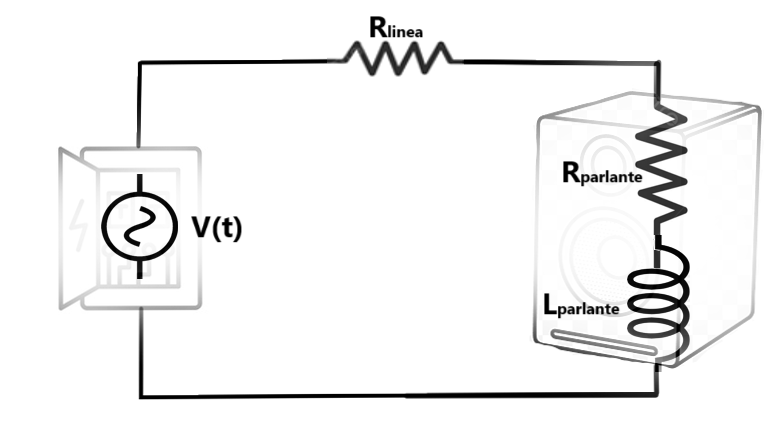
\includegraphics[width=0.5\textwidth]{img/Modelo del circuito.png} % Cambia la ruta a tu imagen
    \caption{Modelo del circuito con el parlante y tablero de Distrubución.}
    \label{fig:mi_imagen}
\end{figure}
        
\section{Porcentajes de Error Para Cada Frecuencia de Muestreo}
A continuacion se presenta el porcentaje de error para cada una de las frecuncias de muestreo.

    \begin{tabular}{ccccc}
        \toprule
        \textbf{Parametro} & \textbf{Error[\%] $f_{\text{100Hz}}$} & \textbf{Error[\%] $f_{\text{180Hz}}$}\\
        \midrule
        Vrms                  & 8.0124   & 0  \\                     
        Irms                  & 19.761  & 0  \\
        P                     & 33.14      & 0  \\
        Q                     & 15.793 & 0 \\
        S                     & 29.36  & 0 \\
        FP                    & 22.68  & 0 \\
        $P_{\text{parlante}}$ & 32.917      & 0  \\
        \bottomrule
        \end{tabular}

    \begin{tabular}{ccc}
        \toprule
        \textbf{Error[\%] $f_{\text{200Hz}}$} & \textbf{Error[\%] $f_{\text{240Hz}}$} & \textbf{Error[\%] $f_{\text{280Hz}}$} \\
        \midrule
        8.0124 & 0 & 6.066 \\ 
        6.5589 & 0 & 4.9577 \\
        16.665 & 0 & 12.492 \\
        1.3999 & 0 & 0.78514 \\
         15.101 & 0 & 11.325 \\
         13.12 & 0 & 10.18 \\
         16.738 & 0 & 12.558   \\
        \bottomrule
        \end{tabular}

        \section{Comparación de procesos de muestreo}
    Para los casos en los cuales se emplearon frecuencias de muestreo de 240 Hz y 180 Hz son los mas eficaces puesto que solo emplean una sola ventana de observación para realizar la estimación de los parámetros de la señal, en cambio en las señales de 280 Hz y 200 Hz se realizan de otra ventana de observación incluyendo las dos en las que se tomo la medición además requerían de 5 y 4 medidas adicionales respectivamente.\\ 

\section{Relación con el Teorema de Nyquist-Shannon}
El teorema de Nyquist-Shannon establece que, para evitar el aliasing y permitir la reconstrucción perfecta de una señal, la frecuencia de muestreo debe ser al menos el doble de la frecuencia máxima de la señal.
\begin{equation}
    f_s \geq 2 f_{\text{máx}}
\end{equation}

\section{Conclusiones y Recomendaciones}
La frecuencia de muestreo tiene un impacto significativo en la estimación de parámetros en sistemas eléctricos. La correcta elección de esta frecuencia, fundamentada en el teorema de Nyquist-Shannon, asegura que la información crítica de la señal sea capturada de manera precisa y que se minimicen los efectos del aliasing. En conclusión, para obtener mediciones confiables y precisas, es esencial seleccionar una frecuencia de muestreo que no solo cumpla con la condición de Nyquist, sino que también considere la naturaleza y dinámica del sistema en estudio.


    \end{document}  
